%%%%%%%%%%%%%%%%%%%%%%%%%%%%%%%%%%%%%%%%%%%%%%%%%%%%%%%%
% Refactored KOMA-Script CV - Single Column (Final Corrected Version)
% Based on user's template, professionally revised.
% by a Job Hunting Expert
%%%%%%%%%%%%%%%%%%%%%%%%%%%%%%%%%%%%%%%%%%%%%%%%%%%%%%%%

\documentclass[11pt, a4paper]{scrartcl}

\usepackage[english]{babel}
\usepackage[utf8]{inputenc}
\usepackage[T1]{fontenc}
\usepackage{lato} % A clean, modern sans-serif font
\usepackage[protrusion=true, expansion=true]{microtype}
\usepackage{amsmath, amsfonts, amsthm}
\usepackage[svgnames]{xcolor}
\usepackage{hyperref}
\usepackage{graphicx}
\usepackage{geometry}
\usepackage{titlesec} % For custom section headers
\usepackage{enumitem} % For custom lists

% --- PAGE & COLOR CONFIGURATION ---
\geometry{
    a4paper,
    left=2cm,
    right=2cm,
    top=2cm,
    bottom=2cm,
    noheadfoot
}
\pagestyle{empty}
\definecolor{sectioncolor}{rgb}{0.0, 0.3, 0.6} % Professional blue

% --- HYPERLINK SETUP ---
\hypersetup{
    colorlinks=true,
    urlcolor=sectioncolor,
    linkcolor=sectioncolor,
    pdfauthor={Min Hu},
    pdftitle={CV of Min Hu}
}

% --- SECTION FORMATTING ---
\titleformat{\section}{\Large\scshape\color{sectioncolor}\raggedright}{}{0em}{}[\titlerule]
\titlespacing{\section}{0pt}{2ex}{1ex}

% --- CUSTOM COMMANDS ---
\newcommand{\workentry}[4]{%
    \noindent\textbf{#2} \hfill \textit{\color{gray} #1} \\
    \textit{#3} \\
    \vspace{0.5ex}
    \noindent\hangindent=1.5em\hangafter=0 \small #4 \normalsize\par
    \vspace{1.5ex}
}

\newcommand{\educationentry}[4]{%
    \noindent\textbf{#2} \hfill \textit{\color{gray} #1} \\
    \textit{#3} \\
    \vspace{0.5ex}
    \noindent\hangindent=1.5em\hangafter=0 \small #4 \normalsize\par
    \vspace{1.5ex}
}

% A robust entry command for skills, etc.
\newcommand{\entry}[2]{%
    \noindent\hangindent=2.5em\hangafter=0
    \parbox{8em}{\textbf{#1}}{#2}\par
    \vspace{0.7ex}
}

% A new command specifically for the awards section layout
\newcommand{\awardentry}[3]{%
    \noindent\textbf{#1} \hfill \textit{\color{gray} #2, #3}\par
    \vspace{1.5ex}
}


\begin{document}

% --- HEADER SECTION ---
\noindent
\begin{minipage}[t]{0.75\linewidth}
    \vspace{0pt} % Aligns the top of the text with the top of the image
    {\Huge\bfseries Min Hu}
    \vspace{1.0ex}
    
    {\large Research Scientist | Biomedical Engineer}
    \vspace{2.0ex}
    
    \small
    \href{mailto:humin.cosmic@gmail.com}{humin.cosmic@gmail.com} \quad\textbar\quad +86 15388077011 \\
    Changsha, China
\end{minipage}%
\hfill%
\begin{minipage}[t]{0.2\linewidth}
    \vspace{0pt} % Aligns the top of the image
    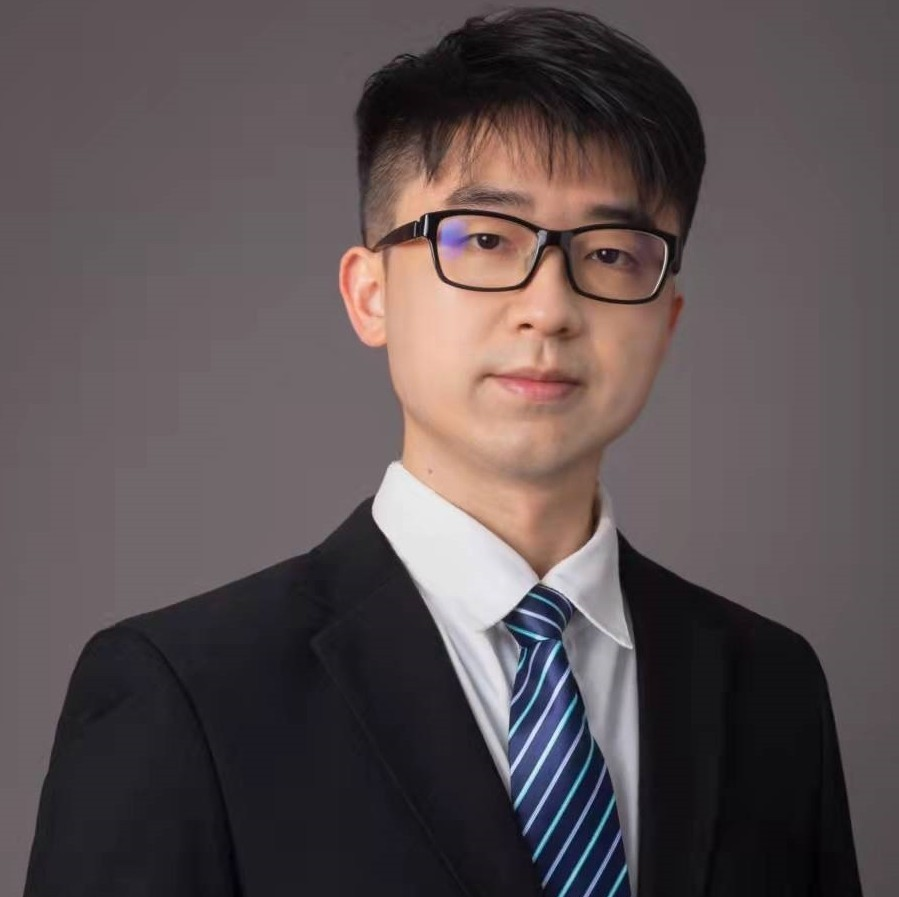
\includegraphics[width=\linewidth, clip]{photo.jpg}
\end{minipage}
\vspace{2ex}


% --- PROFESSIONAL PROFILE ---
\section*{Professional Profile}
\begin{itemize}[leftmargin=1.5em, itemsep=0.5ex]
    \item Research Scientist with a PhD in Medical Informatics and over a decade of experience in applying data science and machine learning to solve complex healthcare challenges.
    \item Proven track record of leading international projects, publishing in high-impact journals (e.g., Computers in Biology and Medicine), and securing patents for novel diagnostic systems.
    \item Expertise in biomedicine, real-world data analysis, and developing clinical decision support systems.
    \item Fluent in English, Japanese, and Mandarin, enabling effective collaboration in global research environments.
\end{itemize}

% --- WORK EXPERIENCE ---
\section*{Work Experience}
\workentry{2023 -- Present}
    {AI Research Scientist}
    {Aier Eye Hospital Group Co., Ltd., Changsha, China}
    {Led research on the application of Multimodal Large Language Models for automated analysis of surgical videos, designing and finetuning a novel framework for the objective evaluation of cataract surgery procedures.
}

\workentry{2021 -- 2023}
    {Postdoctoral Researcher}
    {Aier Eye Hospital Group \& Chinese Academy of Sciences, China}
    {Led research on machine learning applications for ophthalmic imaging data (OCT, fundus) to advance the early detection and prevention of high myopia and dry AMD. }

\workentry{2019 -- 2021}
    {Biomedical Research Engineer}
    {Cosmic Corporation Co., Ltd., Tokyo, Japan}
    {Led a collaborative research project with four public hospitals in Japan to develop a machien learning based clinical decision support system for early thyroid detection using routine laboratory tests. }

% --- EDUCATION ---
\section*{Education}
\educationentry{2015 -- 2019}
    {Ph.D. in Medical Informatics}
    {Kyushu University, Fukuoka, Japan }
    {Research Focus: Real-World Clinical Data Analysis, Data Science, Machine Learning.}

\educationentry{2013 -- 2015}
    {M.S. in Medical Informatics}
    {Kyushu University, Fukuoka, Japan}
    {Research Focus: Medical Sensors, Public Health, Telemedicine.}

\educationentry{2007 -- 2011}
    {B.S. in Biomedical Information Engineering}
    {Northeastern University, Shenyang, China}
    {Relevant Coursework: Computer Science, C++/Java Programming, Data Structures \& Algorithms, Medical Imaging.}

% --- SKILLS & EXPERTISE ---
\section*{Skills \& Expertise}
\entry{Programming}{Python (Pandas, Scikit-learn, PyTorch, TensorFlow), SQL, Linux Systems, Git}
\entry{Expertise}{Computer Science, Data Analysis, Medical Statistics}
\entry{Languages}{Mandarin Chinese (Native), English (TOEIC 950/990), Japanese (JLPT N1)}

% --- PUBLICATIONS ---
\section*{Selected Publications}
{\small
\begin{enumerate}[label={[\arabic*]}, leftmargin=*, itemsep=1ex]
    \item Cao D, \textbf{Hu M} (co-first), Zhi D, Liang J, Tan Q, Lei Q, Dai W. Systematic evaluation of machine learning-enhanced trifocal IOL power selection for axial myopia cataract patients. \textit{Computers in Biology and Medicine}, 2024: 173, 108245. (IF 7.0, Q1).
    \item \textbf{Hu M}, Wu B, Lu D, Xie J, Chen Y, Yang Z, Dai W. Two-step hierarchical neural network for classification of dry age-related macular degeneration using optical coherence tomography images. \textit{Frontiers in Medicine}, 2023:10. (IF 3.9, Q1).
    \item \textbf{Hu M}, Asami C, Iwakura H, Nakajima Y, Sema R, Kikuchi T, Sakakibara Y. Development and preliminary validation of a machine learning system for thyroid dysfunction diagnosis based on routine laboratory tests. \textit{Communications Medicine}, 2022:2(1), 9. (IF 5.4, Q1).
    \item \textbf{Hu M}, Nohara Y, Wakata Y, Ahmed A, Nakashima N, Nakamura M. Machine Learning Based Prediction of Data-driven Approaches...in Bangladesh. \textit{Eur J Bioinformatics} 14.4 2018: 20-28.
    \item \textbf{Hu M}, Nohara Y, Nakamura M, Nakashima N. Prediction and factor extraction of drug function by analyzing medical records in developing countries. \textit{Studies in Health Technology and Informatics}. Vol 245;2017:403-407.
\end{enumerate}
}

% --- PATENTS ---
\section*{Patents}
{\small
\begin{enumerate}[label={[\arabic*]}, leftmargin=*, itemsep=1ex]
    \item \textbf{Hu M}, et al. A Medical Haptic Feedback Clamping Device. China Utility Model Patent, CN220436990U. Granted July 17, 2023.
    \item \textbf{Hu M}, et al. A Haptic Feedback Sensing Control Handle. China Utility Model Patent, CN218204642U. Granted Dec 30, 2022.
    \item \textbf{Hu M}, et al. Operating Pen for a Surgical Haptic Sensing Device. China Design Patent, CN307806509S. Granted Dec 30, 2022.
    \item \textbf{Hu M}, et al. Biological Information Evaluation System and Biological Information Evaluation Program. Japan Invention Patent, JP6948497B2. Granted Sep 24, 2021.
\end{enumerate}
}

% --- RESEARCH FUNDING ---
\section*{Research Funding}
\workentry{2022 -- 2024}
    {Principal Investigator}
    {Application of Digital 3D Eye Model in Cataract Surgery Training}
    {Grant No. AF2202D12}

\workentry{2021 -- 2023}
    {Major Contributor}
    {Development and Application of Audiovisual-Haptic Interaction Technology for Remote Ophthalmic Surgery}
    {Grant No. 2021GK4015}
    
% --- AWARDS ---
\section*{Awards}
\awardentry{Key Professional in the Big Health Industry}{2023}{China}
\awardentry{Xingcheng Cup Technological Innovation Competition}{2022}{China}
\awardentry{MEXT Scholarship for Doctoral Studies}{2015}{Japan}

\end{document}